\section{选取特征进行实验}
该部分进行的实验:用Matlab和C(以MATLAB为主)实现对浮游动物特征的提取(特征包括PkID中部分特征以及计算视觉中的一些特征提取方法),并进行分类。在该实验中使用的去噪方法是去掉连通区域小于50的噪声。

%\begin{comment}
%\subsubsection{实验一}
%\begin{description}
%\item[去噪方法:] 去掉连通区域小于20的噪声。
%\item[选用特征:] Mean、StdDev、CV、SR、MeanPos、Elongation、Circ、Feret、PerimAreaexc、CDexc、Skelarea、FeretAreaexc、PerimFeret、矩形度、体态比、凸率、伸长度、灰度共生矩阵(对比度)、对称性(左右),前13个特征为PkID系统中使用的部分特征。
%\item[分类器:] 采用随机森林进行训练和分类得到的结果如图~\ref{fig:19-Features-MATLAB-our-RF},其分类准确率为71.9\%。采用SVM Linear进行训练和分类得到的结果如图~\ref{fig:19-Features-MATLAB-our-SVM-Linear},其分类准确率为58.4\%
%\end{description}
%\begin{figure}[!ht]
%\centering
%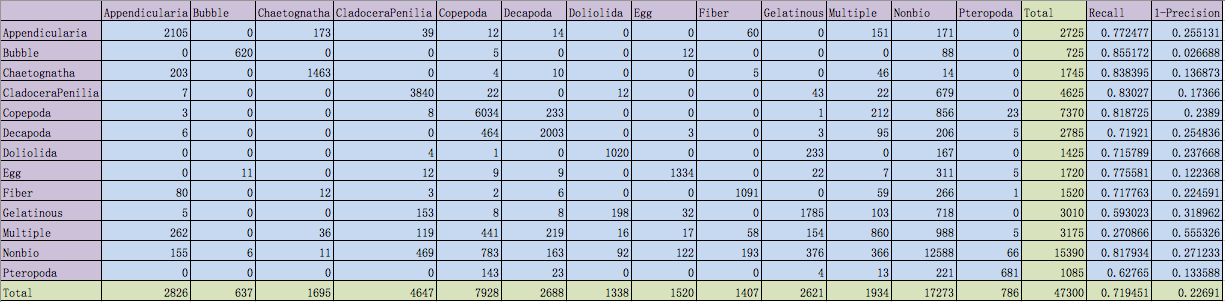
\includegraphics[width=1.0\linewidth]{19-Features-MATLAB-our20-RF}
%\caption{Matlab-19个特征采用随机森林进行分类的结果}
%\label{fig:19-Features-MATLAB-our20-RF}
%\end{figure}
%
%\begin{figure}[!ht]
%\centering
%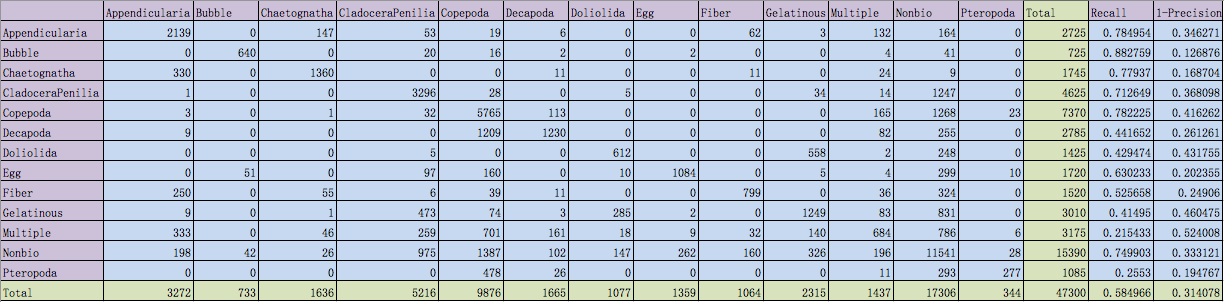
\includegraphics[width=1.0\linewidth]{19-Features-MATLAB-our20-SVM-Linear}
%\caption{Matlab-19个特征采用SVM Linear进行分类的结果}
%\label{fig:19-Features-MATLAB-our20-SVM-Linear}
%\end{figure}
%\end{comment}
\subsection{参数特征选取实验}
\subsubsection{实验一}
\begin{description}
\item[选用特征:] Mean、StdDev、CV、SR、MeanPos、Elongation、Circ、Feret、PerimAreaexc、CDexc、Skelarea、FeretAreaexc、PerimFeret。(这些特征是从PkID67个特征中选取的)
\item[分类器:] 随机森林、SVM
\end{description}
\begin{itemize}
\item MATLAB:采用随机森林进行训练和分类得到的结果如图~\ref{fig:13-Features-MATLAB-our-RF},其分类准确率为61.6\%。采用SVM Linear进行训练和分类得到的结果如图~\ref{fig:13-Features-MATLAB-our-SVM-Linear},其分类准确率为39.9\%
\item C:采用随机森林进行训练和分类得到的结果如图~\ref{fig:13-Features-C-our-RF},其分类准确率为59.7\%。采用SVM Linear进行训练和分类得到的结果如图~\ref{fig:13-Features-C-our-SVM-Linear},其分类准确率为33.4\%
\end{itemize}

\begin{figure}[!ht]
\centering
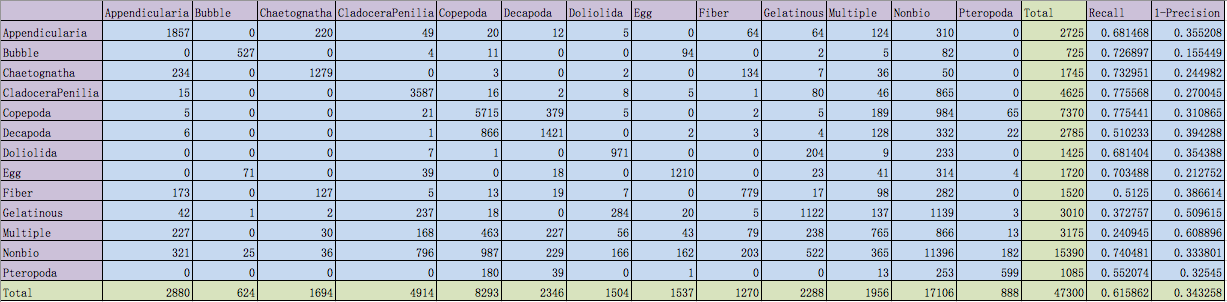
\includegraphics[width=1.0\linewidth]{13-Features-MATLAB-our-RF}
\caption{Matlab-13个特征采用随机森林进行分类的结果}
\label{fig:13-Features-MATLAB-our-RF}
\end{figure}

\begin{figure}[!ht]
\centering
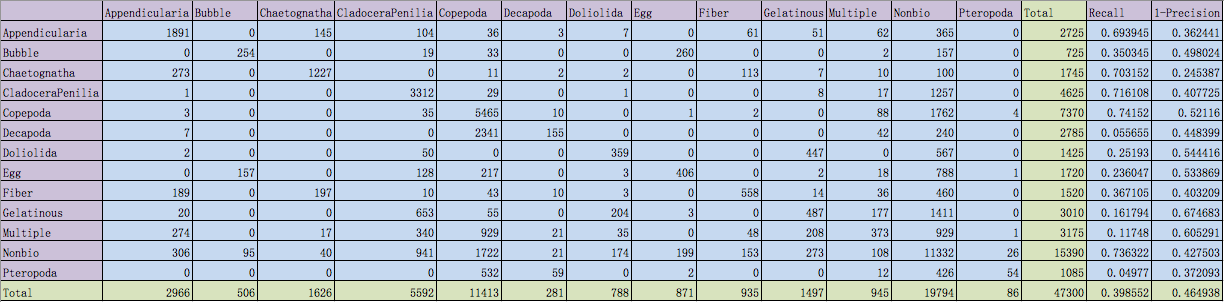
\includegraphics[width=1.0\linewidth]{13-Features-MATLAB-our-SVM-Linear}
\caption{Matlab-13个特征采用SVM Linear进行分类的结果}
\label{fig:13-Features-MATLAB-our-SVM-Linear}
\end{figure}

\begin{figure}[!ht]
\centering
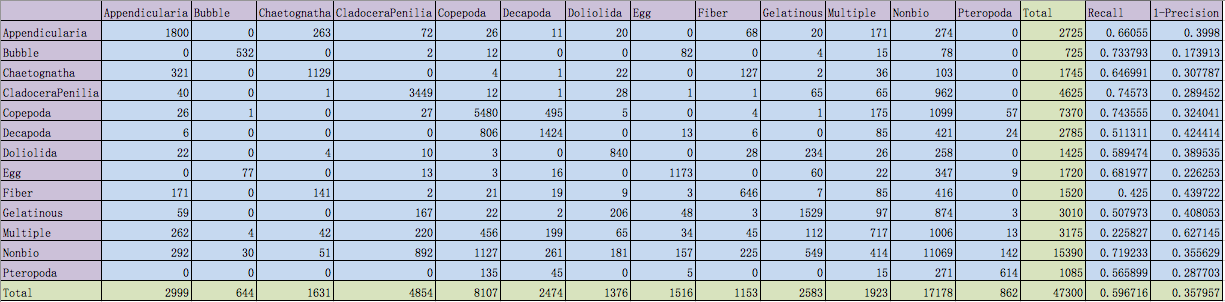
\includegraphics[width=1.0\linewidth]{13-Features-C-our-RF}
\caption{C-13个特征采用随机森林进行分类的结果}
\label{fig:13-Features-C-our-RF}
\end{figure}

\begin{figure}[!ht]
\centering
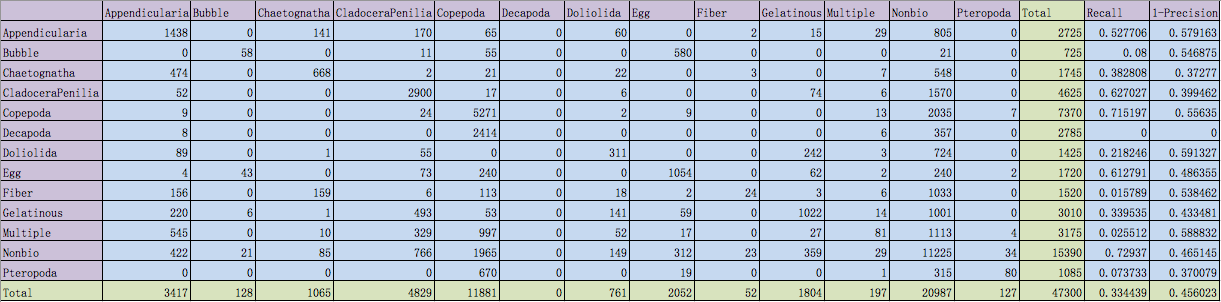
\includegraphics[width=1.0\linewidth]{13-Features-C-our-SVM-Linear}
\caption{C-13个特征采用SVM Linear进行分类的结果}
\label{fig:13-Features-C-our-SVM-Linear}
\end{figure}
%根据实验一、二的分析:去掉小连通区域的噪声可以提高分类准确率,但是去掉的小连通区域面积阈值设置相差不大时不会对实验结果产生很大影响。

\subsubsection{实验二}
\begin{description}
\item[选用特征:] Mean、StdDev、CV、SR、MeanPos、Elongation、Circ、Feret、PerimAreaexc、CDexc、Skelarea、FeretAreaexc、PerimFeret、矩形度、体态比、凸率、伸长度、灰度共生矩阵(对比度)、对称性(左右)。(前13个特征为PkID系统中的部分特征)
\item[分类器:] 随机森林、SVM

MATLAB:采用随机森林进行训练和分类得到的结果如图~\ref{fig:19-Features-MATLAB-our-RF},其分类准确率为72.9\%。采用SVM Linear进行训练和分类得到的结果如图~\ref{fig:19-Features-MATLAB-our-SVM-Linear},其分类准确率为58.9\%
\end{description}
\begin{figure}[!ht]
\centering
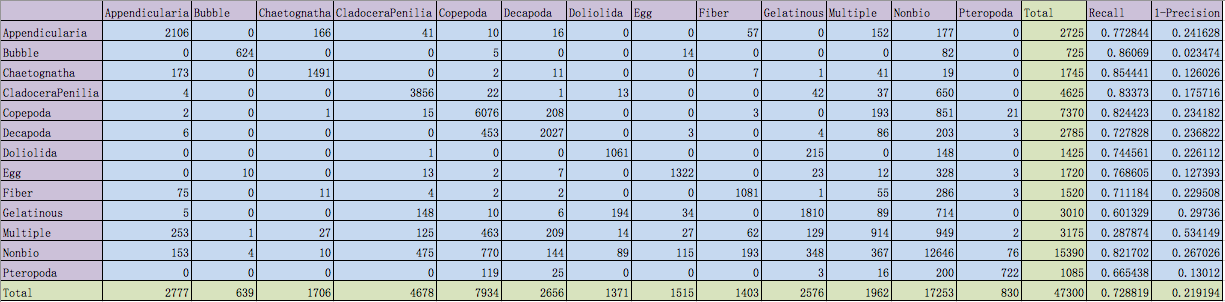
\includegraphics[width=1.0\linewidth]{19-Features-MATLAB-our-RF}
\caption{Matlab-19个特征采用随机森林进行分类的结果}
\label{fig:19-Features-MATLAB-our-RF}
\end{figure}

\begin{figure}[!ht]
\centering
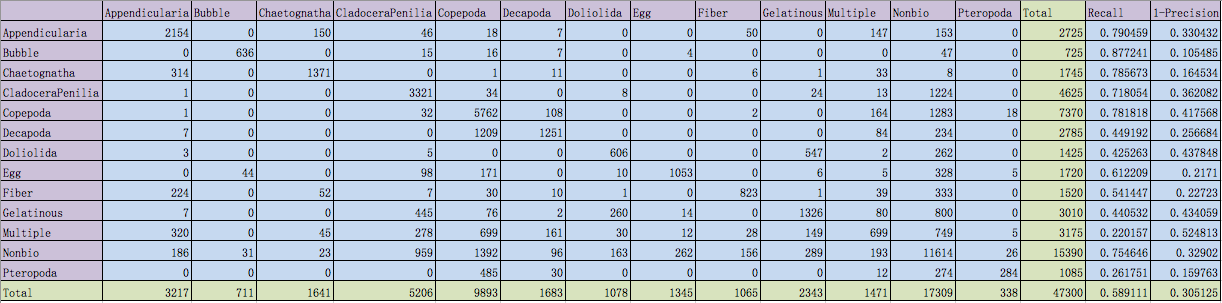
\includegraphics[width=1.0\linewidth]{19-Features-MATLAB-our-SVM-Linear}
\caption{Matlab-19个特征采用SVM Linear进行分类的结果}
\label{fig:19-Features-MATLAB-our-SVM-Linear}
\end{figure}
%根据实验一、二的分析:去掉小连通区域的噪声可以提高分类准确率,但是去掉的小连通区域面积阈值设置相差不大时不会对实验结果产生很大影响。

\subsubsection{实验三}
\label{shiyan3}
\begin{description}
\item[选用特征:] 在实验一、二所用特征的基础上增加的了不变矩特征。
\item[分类器:] 随机森林、SVM

MATLAB:采用随机森林进行训练和分类得到的结果如图~\ref{fig:20-Features-MATLAB-our-RF},其分类准确率为73.7\%。采用SVM Linear进行训练和分类得到的结果如图~\ref{fig:20-Features-MATLAB-our-SVM-Linear},其分类准确率为61.0\%
\end{description}
\begin{figure}[!ht]
\centering
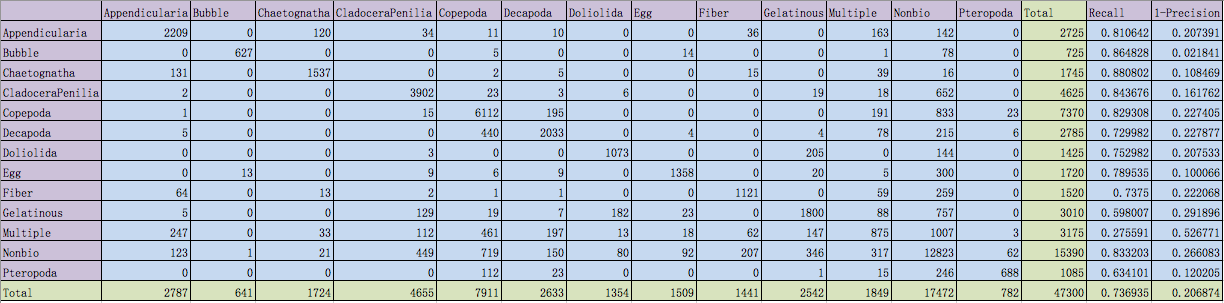
\includegraphics[width=1.0\linewidth]{20-Features-MATLAB-our-RF}
\caption{Matlab-20个特征采用随机森林进行分类的结果}
\label{fig:20-Features-MATLAB-our-RF}
\end{figure}

\begin{figure}[!ht]
\centering
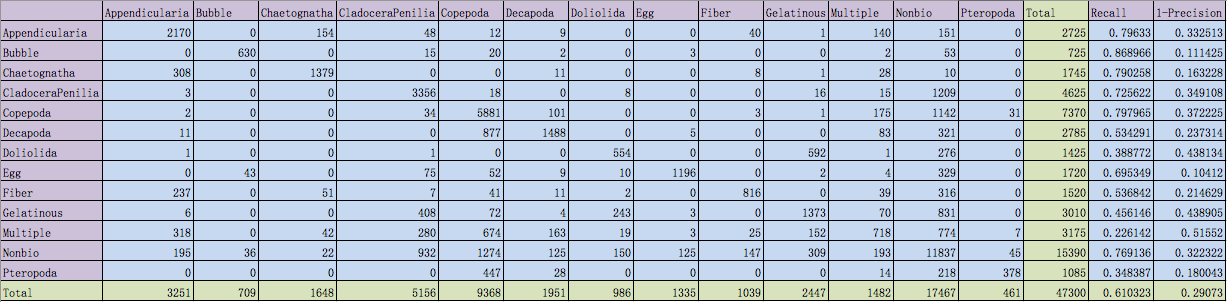
\includegraphics[width=1.0\linewidth]{20-Features-MATLAB-our-SVM-Linear}
\caption{Matlab-20个特征采用SVM Linear进行分类的结果}
\label{fig:20-Features-MATLAB-our-SVM-Linear}
\end{figure}

\subsection{特征融合方法实验}
\subsubsection{实验一(特征融合方法一)}
\label{ronghe1}
该实验进行的是特征融合。由于在实验一——三中使用的特征都是特征值,而HOG、LBP以及一些形状特征都是特征向量的形式。如果要将这些特征一起使用就需要进行特征融合。在该实验中,将\ref{shiyan3}中的20个特征和LBP特征融合,具体的融合方法:
\begin{enumerate}
\item 用训练集不同种的特征(这里的将特征分为两种:实验三种的20个特征和LBP特征)分别进行训练得到分类器(20个特征采用随机森林进行训练,LBP采用SVM进行训练)。然后将训练集对应的这两种特征分别输入到其对应的分类器中进行预测,这两种特征会分别得到属于每个类别的分类概率($m \times n$维,m为训练集样本数,n为类别数)。
\item 将每种特征得到的概率进行拼接($m \times 2n$维),再输入到分类器(这里的分类器使用的是SVM)进行训练。
\item 然后将测试集的分类概率(用和1中的方法可以得到测试集的分类概率)输入到训练好的分类器中,得到最终的分类结果。
\end{enumerate}

在该实验得到的分类结果如图\ref{fig:20+LBP-fusion1-matlab},其分类准确率为76.1\%。
\begin{figure}[!ht]
\centering
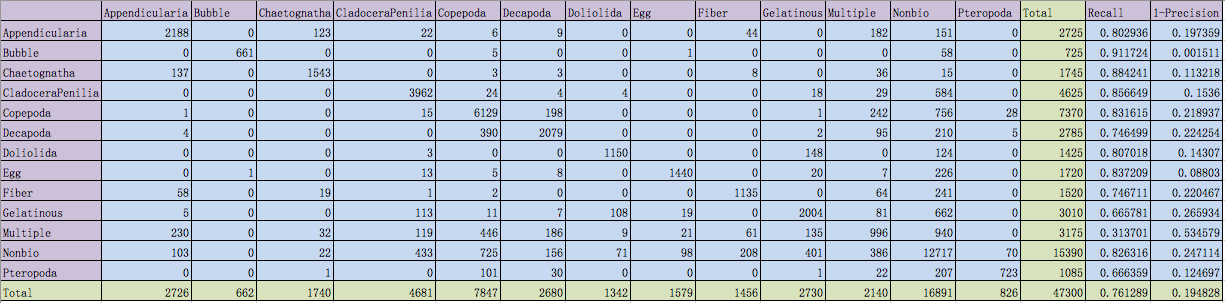
\includegraphics[width=1.0\linewidth]{20+LBP-fusion1-matlab}
\caption{Matlab-20个特征和LBP特征融合方法一}
\label{fig:20+LBP-fusion1-matlab}
\end{figure}

\subsubsection{实验二(特征融合方法二)}
该实验也是将\ref{shiyan3}中的20个特征和LBP特征融合,采用的融合方法:
\begin{enumerate}
\item 用训练集不同种的特征(这里的将特征分为两种:实验三种的20个特征和LBP特征)分别进行训练得到分类器(20个特征采用随机森林进行训练,LBP采用SVM进行训练)。
\item 计算每个分类器的权重:对于训练样本集中的每一个样本,分别将其每种特征输入到对应的特征分类器中进行识别,如果能够识别正确,则其对应的特征分类器的权重加一,最终得到每种特征的权重。
\item 预测概率:每幅的不同种类特征通过分类器可以得到其属于每个类别的分类概率(与实验四中步骤1相同)。根据权重和分类概率,计算出最终属于各个类别的概率。
\end{enumerate}

在该实验得到的分类结果如图\ref{fig:20+LBP-fusion2-matlab},其分类准确率为73.7\%。
\begin{figure}[!ht]
\centering
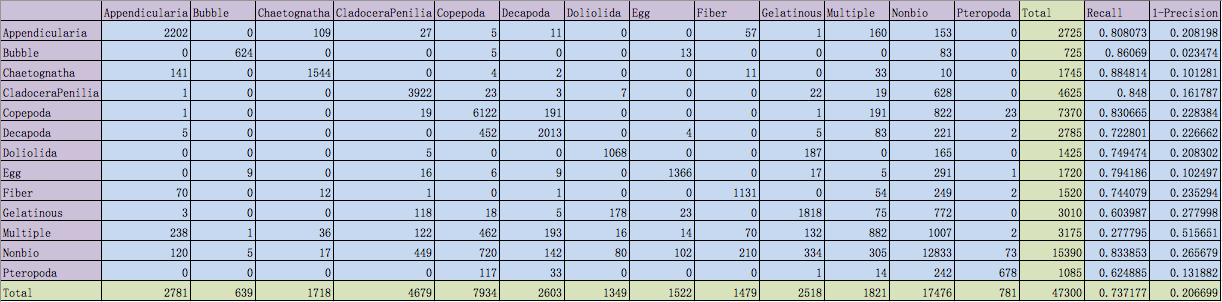
\includegraphics[width=1.0\linewidth]{20+LBP-fusion2-matlab}
\caption{Matlab-20个特征和LBP特征融合方法二}
\label{fig:20+LBP-fusion2-matlab}
\end{figure}

\subsection{融合不同特征实验}
该部分采用的分类器为SVM和随机森林。
\subsubsection{实验一}
\begin{description}
\item[选用特征:] 在\ref{ronghe1}所用特征的基础上融合Gabor特征(采用特征融合方法一)。
\end{description}
MATLAB:在该实验得到的分类结果如图\ref{fig:20+LBP+Gabor-Features-MATLAB},其分类准确率为73.6\%。
\begin{figure}[!ht]
\centering
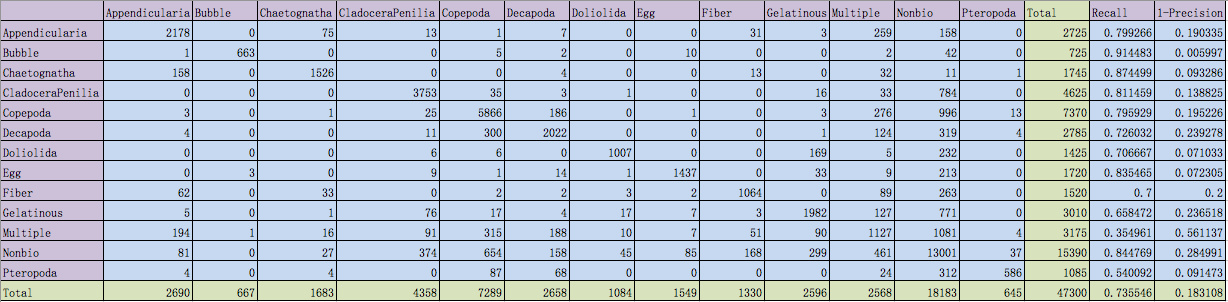
\includegraphics[width=1.0\linewidth]{20+LBP+Gabor-Features-MATLAB}
\caption{Matlab-20个特征、LBP和Gabor特征融合方法一}
\label{fig:20+LBP+Gabor-Features-MATLAB}
\end{figure}

\subsubsection{实验二}
\begin{description}
\item[选用特征:] 在\ref{ronghe1}所用特征的基础上融合Fourier描述子(采用特征融合方法一)。
\end{description}
MATLAB:在该实验得到的分类结果如图\ref{fig:20+LBP+Fourier-Features-MATLAB},其分类准确率为76.2\%。
\begin{figure}[!ht]
\centering
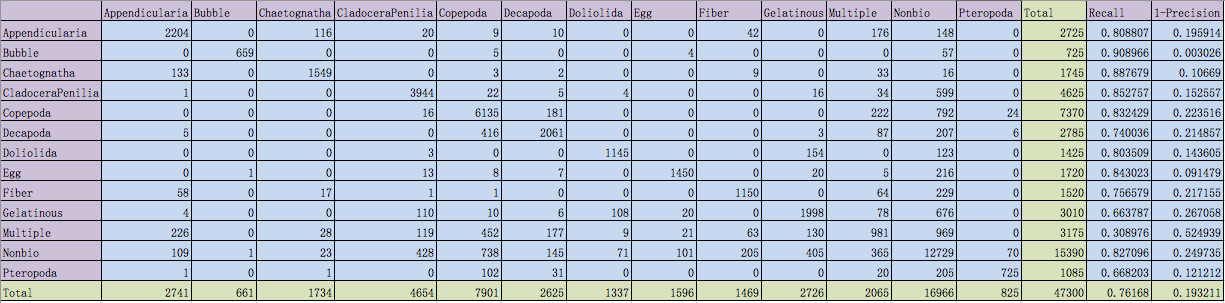
\includegraphics[width=1.0\linewidth]{20+LBP+Fourier-Features-MATLAB}
\caption{Matlab-20个特征、LBP和Fourier描述子融合方法一}
\label{fig:20+LBP+Fourier-Features-MATLAB}
\end{figure}

\subsubsection{实验三}
\begin{description}
\item[选用特征:] 在\ref{ronghe1}所用特征的基础上融合SIFT特征(采用特征融合方法一)。
\end{description}
MATLAB:在该实验得到的分类结果如图\ref{fig:20+LBP+SIFT-Features-MATLAB},其分类准确率为76.2\%。
\begin{figure}[!ht]
\centering
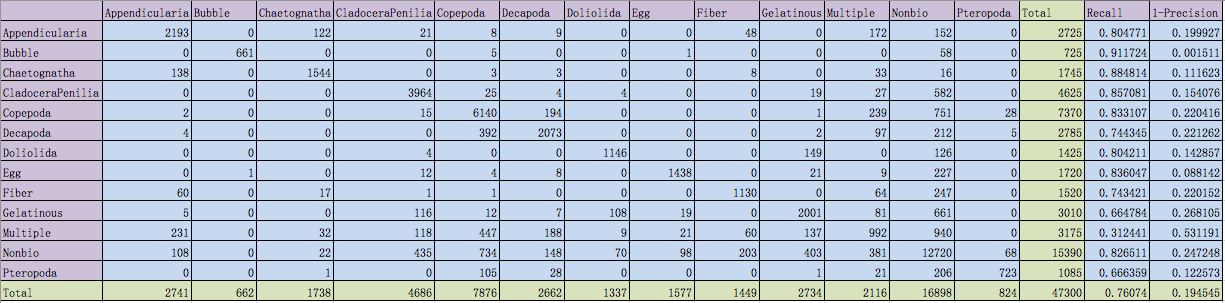
\includegraphics[width=1.0\linewidth]{20+LBP+SIFT-Features-MATLAB}
\caption{Matlab-20个特征、LBP和SIFT特征融合方法一}
\label{fig:20+LBP+SIFT-Features-MATLAB}
\end{figure}


\subsection{ELM作为分类器的实验}
该部分使用极限学习机(ELM)作为分类器。

\subsubsection{实验一}
\begin{description}
\item[选用特征:] 采用\label{shiyan3}中的20个特征进行实验。
\end{description}
MATLAB:在该实验中ELM隐藏神经元设置为650个,实验得到的分类结果如图\ref{fig:20-Features-ELM-MATLAB},其分类准确率为72.4\%。
\begin{figure}[!ht]
\centering
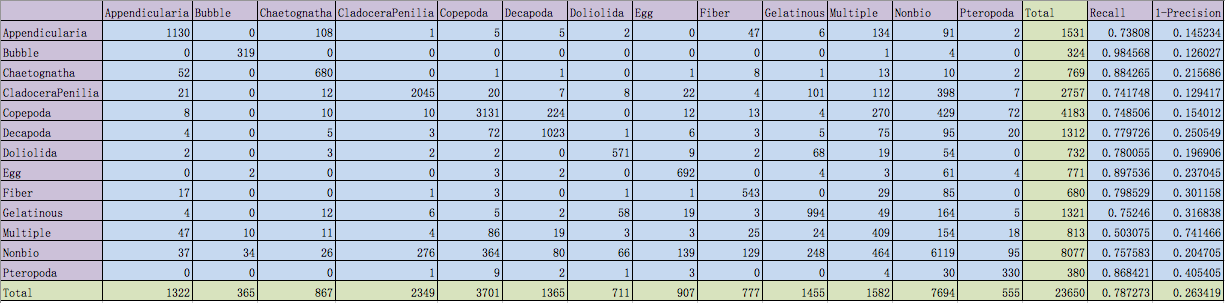
\includegraphics[width=1.0\linewidth]{20-Features-ELM-MATLAB}
\caption{Matlab-20个特征采用ELM进行分类}
\label{fig:20-Features-ELM-MATLAB}
\end{figure}


\section{实验总结}
实验总结:
\begin{itemize}
\item MATLAB进行实验的结果要比C的好,因此实验以MATLAB为主。
\item 在进行实验过程中,PKID中的特征只使用了13个(原来计划选用22个)。原因是由于图像质量原因,特征提取效果不是特别好,以至于一些特征对分类准确率的提升没有太大贡献。另外,还有两个特征我没有找到计算方法,但我感觉对实验结果提高不会有太大影响。
\item 实验中提取的特征不如PkID系统中的特征好(有一部分原因是实验中特征提取是对图像提取的,而图像质量又较低,导致提取的特征不准确。PkID系统中的基本特征都是从ZooProcess中得到的,能更好的反映浮游动物的特征),其分类的准确率也比PkID系统中的特征低2到3个百分点。
\item 因为需要使用的特征既有特征值,也有特征向量,这些特征直接一起使用会降低准确率,因此需要进行了特征融合(实验四、五)。目前采用了20个特征与LBP特征融合,分类的准确率有了一定的提高(达到76.1\%)。
\end{itemize}

接下来的工作:在特征融合的基础上继续进行实验,实验将不同形式的特征结合来得到更高的分类准确率。
